\documentclass[12pt,a4paper]{ctexart}
\usepackage{amsmath,amssymb}
\usepackage[margin=2.5cm]{geometry}
\usepackage{graphicx}

\newcommand{\blank}[1][3cm]{\underline{\hspace{#1}}}
\newcommand{\answer}{\par\vspace{0.5em}\noindent\rule{\linewidth}{0.4pt}\par\vspace{1em}}

% 图片占位框：高度 5cm，宽度 0.8\linewidth，可自行改
\newcommand{\imgslot}[1][0.8\linewidth]{%
  \begin{center}
  \fbox{\begin{minipage}[c][5cm][c]{#1}\centering 图片占位\end{minipage}}
  \end{center}
}

\begin{document}

\section*{Prob-1}

模型：
\[
y_i = \beta_0 + \beta_1 x_i + \varepsilon_i,\quad
E(\varepsilon_i)=0,\quad Var(\varepsilon_i)=\sigma^2,\quad Cov(\varepsilon_i,\varepsilon_j)=0.
\]

记
\[
S_{xx}=\sum_{i=1}^n (x_i-\bar{x})^2,\qquad
S_{xy}=\sum_{i=1}^n (x_i-\bar{x})(y_i-\bar{y}).
\]

OLS 估计量：
\[
\hat{\beta}_1=\frac{S_{xy}}{S_{xx}},\qquad
\hat{\beta}_0=\bar{y}-\hat{\beta}_1\bar{x}.
\]

等价地：
\[
\hat{\beta}_1=\beta_1+\frac{\sum_{i=1}^n (x_i-\bar{x})\varepsilon_i}{S_{xx}},
\]
\[
\hat{\beta}_0=\beta_0+\bar{\varepsilon}-\bar{x}\cdot
\frac{\sum_{i=1}^n (x_i-\bar{x})\varepsilon_i}{S_{xx}}.
\]

由 \(E(\varepsilon_i)=0\)，得
\[
E(\hat{\beta}_1)=\beta_1,\qquad E(\hat{\beta}_0)=\beta_0.
\]

\[
Var(\hat{\beta}_1)
=\frac{\sum_{i=1}^n (x_i-\bar{x})^2 Var(\varepsilon_i)}{S_{xx}^2}
=\frac{\sigma^2 S_{xx}}{S_{xx}^2}
=\frac{\sigma^2}{S_{xx}}.
\]

将 \(\hat{\beta}_0-\beta_0\) 写成
\[
\hat{\beta}_0-\beta_0=
\sum_{i=1}^n \left[
\frac{1}{n}-\frac{\bar{x}(x_i-\bar{x})}{S_{xx}}
\right]\varepsilon_i,
\]
则
\[
Var(\hat{\beta}_0)
=\sigma^2\sum_{i=1}^n
\left[
\frac{1}{n}-\frac{\bar{x}(x_i-\bar{x})}{S_{xx}}
\right]^2
=\sigma^2\left(\frac{1}{n}+\frac{\bar{x}^2}{S_{xx}}\right).
\]

\answer

\section*{Prob-2}
设
\[
y_i=\beta_0+\beta_1 x_i+\varepsilon_i,\qquad
\varepsilon_i\sim N(0,\sigma^2),\quad \text{i.i.d.}
\]

似然函数为
\[
L(\beta_0,\beta_1,\sigma^2)
=(2\pi\sigma^2)^{-n/2}
\exp\left[-\frac{1}{2\sigma^2}
\sum_{i=1}^n (y_i-\beta_0-\beta_1 x_i)^2\right].
\]

对数似然为
\[
\ell=\ln L
=-\frac{n}{2}\ln(2\pi)
-\frac{n}{2}\ln\sigma^2
-\frac{1}{2\sigma^2}
\sum_{i=1}^n (y_i-\beta_0-\beta_1 x_i)^2.
\]

固定 \(\sigma^2\) 时，最大化 \(\ell\) 等价于最小化
\[
\sum_{i=1}^n (y_i-\beta_0-\beta_1 x_i)^2,
\]
因此 \(\beta_0,\beta_1\) 的 MLE 与 OLS 相同：
\[
\hat{\beta}_1^{MLE}
=\frac{\sum_{i=1}^n (x_i-\bar{x})(y_i-\bar{y})}
{\sum_{i=1}^n (x_i-\bar{x})^2},
\qquad
\hat{\beta}_0^{MLE}=\bar{y}-\hat{\beta}_1^{MLE}\bar{x}.
\]

对 \(\sigma^2\) 求偏导并令其为零：
\[
\frac{\partial \ell}{\partial \sigma^2}
=-\frac{n}{2\sigma^2}
+\frac{1}{2\sigma^4}
\sum_{i=1}^n (y_i-\beta_0-\beta_1 x_i)^2=0.
\]
代入 \(\hat{\beta}_0,\hat{\beta}_1\)，得
\[
\hat{\sigma}^2_{MLE}
=\frac{1}{n}
\sum_{i=1}^n (y_i-\hat{\beta}_0-\hat{\beta}_1 x_i)^2
=\frac{RSS}{n}.
\]

因此
\[
\hat{\beta}_0^{MLE}=\hat{\beta}_0^{OLS},\qquad
\hat{\beta}_1^{MLE}=\hat{\beta}_1^{OLS},\qquad
\hat{\sigma}^2_{MLE}=\frac{RSS}{n}.
\]
注意 \(\hat{\sigma}^2_{MLE}\) 是有偏的，无偏估计为
\[
\hat{\sigma}^2=\frac{RSS}{n-2}.
\] 
\answer

\section*{Prob-3}
X=0时，Y的估计值为0，回归线过原点

a.\[
{\beta}_1=\frac{\sum_{i=1}^n x_iy_i}{\sum_{i=1}^n x_i^2},
\]

b.
\[
L(\beta_1,\sigma^2)
=(2\pi\sigma^2)^{-n/2}
\exp\left[-\frac{1}{2\sigma^2}
\sum_{i=1}^n (y_i-\beta_1 x_i)^2\right].
\]
通过同上方法得到结果与LSE相同

c.设 \(Y_i=\beta_1 X_i+\varepsilon_i\)，\(\varepsilon_i\) 独立且 \(E(\varepsilon_i)=0\)。
MLE 为
\[
\hat{\beta}_1=\frac{\sum_{i=1}^n X_iY_i}{\sum_{i=1}^n X_i^2}.
\]
于是
\[
E(\hat{\beta}_1)
=\frac{\sum_{i=1}^n X_iE(Y_i)}{\sum_{i=1}^n X_i^2}
=\frac{\sum_{i=1}^n X_i(\beta_1 X_i)}{\sum_{i=1}^n X_i^2}
=\frac{\beta_1\sum_{i=1}^n X_i^2}{\sum_{i=1}^n X_i^2}
=\beta_1.
\]
故 \(\hat{\beta}_1\) 无偏。
\answer

\section*{Prob-4}
a.误差分布没有确认，故无法得到
b.\[\hat{y}=\beta_0+\beta_1X=200\]
\[\sigma=5\]
Thus, by normality assumption, \[p=68.27\%\]

\section*{Prob-5}
\answer
a.observational

b.Not exactly. Correlation does not imply causation.

c.身体健康状况，经济情况

d.改为实验性研究
\answer

\section*{Prob-6}
a.\[\beta_0=2.1140,\quad \beta_1=0.0388\]
b.\begin{center}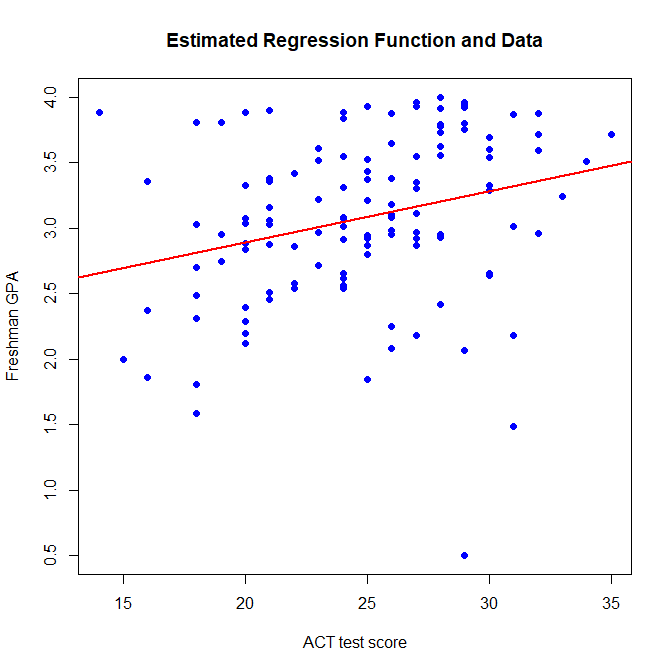
\includegraphics[width=0.8\linewidth]{image.png}\end{center}
No, the residuals seem very large.

c.\[\hat{Y}=2.1140+0.0388*30=3.278\]

d. 0.0388
\answer
\end{document}